%%% -*-LaTeX-*-

\chapter{Current Benchmarks}

This chapter introduces several experiment designs and provides benchmarks for their performance as measured using the current approach to sampling, as well as using other available sampling tools. The implementation strategy of each tool will also be discussed lightly, in order to demonstrate shortcomings when sampling solutions to formulae with factorial solution spaces. These results should be convincing of the need for an alternative approach to the problem, as the current method cannot cope with the scale of the solution spaces in question.

\section{Experiments}


Multiple tools will be applied to solve or sample solutions to formulae reprsenting several experimental designs of increasing complexity comparable to realistic experiments written by current researchers. Table \ref{tab:benchmark_experiments} enumerates the characteristics of each design, including its complexity tier (as defined in chapter 2), properties of its CNF encoding, and a solution count.

For \texttt{stroop-2} and \texttt{stroop-3}, the solution count is precise, as computed by a SAT model counter. For all other experiments, the solution count is approximated as the factorial of the sequence length, as model counters were unable to provide a count in reasonable amount of time. These approximate solution counts ignore both constraints, which would reduce the solution count, and independent factors, which would increase the solution count. In practice, independent factors contribute more solutions than constraints remove.

% NOTE: Stroop tests are with n colors, and a no more than 1 con in a row constraint
\begin{table}[t]
  \centering
  \caption{Benchmark Experiments}
\begin{tabular}{|c|c|c|c|c|c|}
\hline
\multicolumn{1}{|l|}{Experiment Name} & Tier  & Sequence Length & Variables  & Clauses    & Total Solutions    \\ \hline
stroop-2                              & 3     & 4               & 392        & 1,559      & 12                 \\ \hline
stroop-3                              & 3     & 9               & 1,965      & 8,531      & 151,200            \\ \hline
stroop-4                              & 3     & 16              & 3,848      & 16,451     & $\approx 2^{44}$   \\ \hline
stroop-5                              & 3     & 25              & 10,326     & 45,991     & $\approx 2^{83}$   \\ \hline
stroop-congruency-balanced            & 4     & 17              & 5,570      & 24,215     & $\approx 2^{48}$   \\ \hline
stroop-response                       & 4     & 33              & 16,242     & 72,679     & $\approx 2^{122}$  \\ \hline
padmala-pessoa                        & 4     & 37              & 116,289    & 559,080    & $\approx 2^{143}$  \\ \hline
task-switching                        & 4     & 32              & 14,246     & 62,700     & $\approx 2^{117}$  \\ \hline
task-switching-2                      & 5     & 146             & 742,832    & 3,672,632  & $\approx 2^{844}$  \\ \hline
task-switching-cue-switching          & 4     & 1,025           & -          & -          & $\approx 2^{8778}$ \\ \hline
\end{tabular}
\label{tab:benchmark_experiments}%
\end{table}


% \subsection{Practical Time Limitations}

% Before proceeding, we will establish the premise that any implementation which counts solutions directly is infeasible due to the time cost. Suppose that a 4GHz CPU were fully employed in simply incrementing a variable $c$ from $0$ to $s$, where $s$ is the total number of solutions for each of the benchmark experiments listed above. We will also assume that the increment instruction requires only a single clock cycle to execute. This CPU could increment $c$ to 4,000,000,000 in a single second. Counting the total number of solutions for the first two experiments would appear to complete instantaneously. For \texttt{stroop-4}, counting would take a bit longer: $\frac{2^{44}}{4,000,000,000} = 4,398$ seconds, or $1.2$ hours. While certainly not snappy, this is still a reasonable amount of time to wait. Moving on to \texttt{stroop-5} however, the wait becomes 76,669,572 years! The time required grows factorially, along with the size of the solution space. It is certain that these tools will be doing much more with each solution than simply incrementing a counter, and will thus require more clock cycles. Therefore, if any of these tools are to be useful, they must employ a strategy that does not require work in proportion to the number of solutions to the formula.


\section{Benchmarks}

This section presents the results of testing multiple SAT solving and sampling tools against the experiments presented previously, as well as additional information on the implemenation strategy of each tool. All sampling benchmarks were configured to generate only 10 samples. All benchmarks were run on a PC running Ubuntu 18.04.2 LTS with 16GB of memory and an 8-core Intel Core i7-7700 at 3.60 GHz.

\subsection{CryptoMiniSat}

CryptoMiniSat \cite{DBLP:conf/sat/SoosNC09,DBLP:conf/sat/2009} is the main SAT solver that SweePea relies on for generating non-uniformly sampled trial sequences. SweetPea achieves this with CryptoMiniSat by using the naive approach of solving for any solution, and then constraining the original formula to disallow that particular solution from being produced a second time. Due to the difficulty encountered while attempting to use SAT samplers, it has proven quite valuable to provide researchers with this ability to quickly generate some number of trial sequences conforming to their design, even though they may not be uniformly distributed. CryptoMiniSat is also used internally by Unigen. Lastly, in addition to logical \texttt{AND}, \texttt{OR}, and \texttt{NOT} clauses, CryptoMiniSat also supports \texttt{XOR} claues, although SweetPea has not yet put these to use. This is an opportunity for improvement. Table \ref{tab:benchmark_experiments_cmsat} denotes the the time required for CryptoMiniSat to compute a single solution to the SAT formula for each experiment.

% python -m timeit "__import__('os').system('cryptominisat5 padmala-pessoa.cnf > /dev/null')"

\begin{table}[t]
  \centering
  \caption{Time to Solve for 1 Solution with CryptoMiniSat}
\begin{tabular}{|c|c|c|c|c|}
\hline
\multicolumn{1}{|l|}{Experiment Name} & Time to Solve (ms)  \\ \hline
stroop-2                              & 4.9                 \\ \hline
stroop-3                              & 9.1                 \\ \hline
stroop-4                              & 18.9                \\ \hline
stroop-5                              & 64.4                \\ \hline
stroop-congruency-balanced            & 23.9                \\ \hline
stroop-response                       & 232                 \\ \hline
padmala-pessoa                        & 3,380               \\ \hline
task-switching                        & 140                 \\ \hline
task-switching-2                      & 200,000             \\ \hline
task-switching-cue-switching          & -                   \\ \hline
\end{tabular}
\label{tab:benchmark_experiments_cmsat}%
\end{table}

The most complicated design for which SweetPea was able to construct a CNF encoding (\texttt{task-switching-2}) took the longest, at 200 seconds. Most other experiments could be solved in less than a second. Since only a single solution is generated, the practical time consideration is of minor importance here.


\subsection{Unigen}

Unigen \cite{chakraborty2013scalable,chakraborty_balancing_2014} is a recently developed SAT \textit{sampler}. Given a boolean formula in conjunctive normal form (CNF), Unigen can produce nearly uniformly sampled satisfying assignments. SweetPea relies directly on Unigen for uniformly sampling trial sequnces for a given design. As explained in chapter 1, the SweetPea encoding is designed such that there is a one-to-one relationship between solutions to the formula, and unique trial sequences that conform to the design. Unigen is based on a hashing technique that partitions the solution space and then samples solutions from each partition. Unigen has worked well for some designs, but its capacities are quickly overwhelmed by even moderately sized designs.

Let $F$ denote a boolean formula in CNF, and let $R_F$ denote the set of satifsying assignments, or witnesses, for $F$. Unigen, as well as several previously developed samplers, are based on a strategy for generating a partition of $R_F$ using a family of 3-independent hash functions which provide strong uniformity guarantees \cite{gomes_near-uniform_2007}. However, there are two obstacles to using this family of functions: First, it requires an additional parameter $m$, which influences the size of the subsets of the partition of $R_F$. Choosing an approparite value for $m$ is non-trivial. Second, these functions rely heavily on the \texttt{XOR} logical operation. Unfortunately, as stated in \cite{chakraborty_balancing_2014}, as the number of variables per \texttt{XOR} clause grows, the difficulty of generating solutions to the formula increases significantly. \cite{Gomes:2007:SXM:1768142.1768155} At the core of Unigen's contributions were techniques for mitigating both of these problems.

\subsubsection{Model Counting}

The best value for $m$ actually depends on $|R_F|$, however in practice this is not known up front. Unigen uses an approximate model counter, ApproxMC \cite{DBLP:journals/corr/ChakrabortyMV13}, to estimate $|R_F|$, from which a narrow range of values for $m$ can be generated and tested for fitness. Unfortunately in practice, ApproxMC has not been able to successfully approximate the count of any of our benchmark experiments beyond \texttt{stroop-3} in a reasonable amount of time, as shown in Table \ref{tab:benchmark_experiments_approxmc}. A new version of ApproxMC was recently published \cite{approxmc_SM19}; however, it relies on the same family of hash functions, so it is unlikely that it will offer significant improvements.

% TODO:
% [appmc] Sampling set size: 160
% [appmc] Sampling var set contains over 100 variables, not displaying
% does approx mc ack that > 100 is infeasible?


\begin{table}[t]
  \centering
  \caption{Time to Compute Approximate Model Count with ApproxMC}
\begin{tabular}{|c|c|}
\hline
\multicolumn{1}{|l|}{Experiment Name} & Time            \\ \hline
stroop-2                              & 5.07ms          \\ \hline
stroop-3                              & 27.4s           \\ \hline
stroop-4                              & Timed Out       \\ \hline
stroop-5                              & Timed Out       \\ \hline
stroop-congruency-balanced            & Timed Out       \\ \hline
stroop-response                       & Timed Out       \\ \hline
padmala-pessoa                        & Timed Out       \\ \hline
task-switching                        & Timed Out       \\ \hline
task-switching-2                      & Timed Out       \\ \hline
task-switching-cue-switching          & -               \\ \hline
\end{tabular}
\label{tab:benchmark_experiments_approxmc}%
\end{table}

In reality, the algorithm implemented by ApproxMC relies on the same family of 3-independent hash functions mentioned previously, therefore it will be subject to the same problem of \texttt{XOR} clause growth, as explained in the next section.

Although available tools struggle to approximate solution counts for SweetPea designs, this is surmountable by estimating $|R_F|$ ourselves using information from the original problem domain. Because each experimental design constructs a sequence of trials based on combinations of factor levels, we can apply techniques for counting sets from combinatorics to estimate $|R_F|$. This will be discussed further in chapter 4.

\subsubsection{XOR Clause Reduction}

Let $X$ be the set of variables in $F$. Using terminology from \cite{chakraborty_balancing_2014}, $X$ is called the \textit{support} of $F$. They observed that there is often a subset $S \subseteq X$, referred to as an \textit{independent support} of $X$, which fully determines all variable assignments for any satisfying assignment. That is, for all satisfying assignments of $F$, there are no two assignments whose values differ only in the assignments of variables $\overline{S}$. In the domain of CRV, $|S|$ is typically significantly smaller than $|X|$, often by many orders of magnitude. Unigen exploits these observations by only applying variables in $S$ to the hash functions, which yields a significant reduction in the number generated XOR clauses. Therefore it is true that Unigen scales to formulae with hundreds of thousands of variables, and even millions of clauses, but \textit{only} when $|S|$ remains small, typically $|S| < 100$. In the Unigen benchmarks, over 200 different formulae were sampled. The largest of these, \texttt{demo3\_new}, had $865,935$ variables and $3,509,158$ clauses, but $|S|$ was only $45$. Similarly, the largest value of $|S|$ in the benchmarks was $78$ in \texttt{diagStencil\_new}, with $94,607$ variables and $2,838,579$ clauses. \cite{chakraborty_parallel_2015}

How does $|S|$ grow in the formulae generated by SweetPea? SweetPea currently selects all variables that directly represent level values for each factor in each trial as the independent support. While this set does not grow factorially, it still quickly grows into the hundreds and thousands, as shown in table \ref{tab:benchmark_experiments_support}. While this indpendent support is certainly not minimal, it is unlikely that improvements to the encoding and the determination of $S$ could scale more than marginally over current performance.

There are a few obvious improvements that could be made. Currently SweetPea is including the variables for \textit{all} factors and levels in the independent support, when in reality only variables for basic factors and derived factors in the crossing need to be included. Additionally, a more efficient encoding could be used based on combinations of variables rather than representing all levels as individual variables. (Although this would increase the complexity of encoding constraints.) Both of these would reduce $|S|$ by some amount, but there is still a theoretical limit by which we are bound. For any formula $F$ with independent support $S$, there are, by definition, at most $2^{|S|}$ solutions to $F$. (In practice the number of solutions will be less, as not \textit{all} possible assignments will satisfy the formula.) If $|S| < 100$ is a practical limit, then even with the most efficient encoding, Unigen would only be able to sample solutions to formulae with at most $2^{100}$ solutions. As seen in Table \ref{tab:benchmark_experiments}, this would allow for marginal scaling, but not generally for all SweetPea designs.

\begin{table}[t]
  \centering
  \caption{Independent Support Size for Benchmark Experiments}
\begin{tabular}{|c|c|}
\hline
\multicolumn{1}{|l|}{Experiment Name}  & $|S|$   \\ \hline
stroop-2                               & 24      \\ \hline
stroop-3                               & 72      \\ \hline
stroop-4                               & 160     \\ \hline
stroop-5                               & 300     \\ \hline
stroop-congruency-balanced             & 270     \\ \hline
stroop-response                        & 526     \\ \hline
padmala-pessoa                         & 1,303   \\ \hline
task-switching                         & 636     \\ \hline
task-switching-2                       & 2,770   \\ \hline
task-switching-cue-switching           & 24,594  \\ \hline
\end{tabular}
\label{tab:benchmark_experiments_support}%
\end{table}


% unigen --verbosity=0 --kappa=0.638 --pivotUniGen=27 --maxLoopTime=3000 --maxTotalTime=36000 --pivotAC=60 --gaussuntil=400 --samples=10 stroop-3.cnf stroop-3-unigen.out
% python -m timeit "__import__('os').system('unigen --verbosity=0 --kappa=0.638 --pivotUniGen=27 --maxLoopTime=3000 --maxTotalTime=36000 --pivotAC=60 --gaussuntil=400 --samples=10 --startIteration=13 stroop-3.cnf stroop3-unigen.out')"

% Time to sample with 10 samples

\begin{table}[t]
  \centering
  \caption{Time to Generate 10 Samples with Unigen}
\begin{tabular}{|c|c|c|c|c|}
\hline
\multicolumn{1}{|l|}{Experiment Name} & Time to Sample  \\ \hline
stroop-2                              & -               \\ \hline
stroop-3                              &            \\ \hline % python -m timeit "__import__('os').system('unigen --verbosity=0 --kappa=0.638 --pivotUniGen=27 --maxLoopTime=3000 --maxTotalTime=36000 --pivotAC=60 --gaussuntil=400 --samples=10 --startIteration=13 stroop-3.cnf
stroop-4                              &        \\ \hline % python -m timeit "__import__('os').system('unigen --verbosity=0 --kappa=0.638 --pivotUniGen=27 --maxLoopTime=3000 --maxTotalTime=36000 --pivotAC=60 --gaussuntil=400 --samples=10 --startIteration=38 stroop-3.cnf
stroop-5                              &        \\ \hline
stroop-congruency-balanced            &        \\ \hline
stroop-response                       &        \\ \hline
padmala-pessoa                        &        \\ \hline
task-switching                        &        \\ \hline
task-switching-2                      &        \\ \hline
task-switching-cue-switching          & -               \\ \hline
\end{tabular}
\label{tab:benchmark_experiments_unigen}%
\end{table}

This shortcoming is proved out in practice, as Unigen fails to count or sample from formulae where $|S| > 100$. Table \ref{tab:benchmark_experiments_unigen} denotes the time required for Unigen to generate 10 samples for each experiment when an estimate for $|R_F|$ is provided manually based on the factorial of the sequence length. Nearly all of them fail to complete in the allotted time. Because Unigen can only effectively sample large formulae when $|S|$ is small, in practice $|S| < 100$, it is insufficient for the needs of SweetPea. Several other samplers were tested as well, but in our experiments, none of them were successful.


\subsection{KUS}

KUS \cite{SGRM18} is another SAT sampling tool developed by some of the same team behind Unigen. However, it approaches the problem quite differently. KUS requires a compiled deterministic decomposable negation normal form (d-DNNF) of a formula in conjunctive normal form. There are known polynomial time techniques for many operations on the d-DNNF representation of a boolean formula, including model counting. KUS takes advantage of these techniques to uniformly sample solutions using this form. This technique offloads much of the complexity to to the d-DNNF compiler, rather than the sampling phase. KUS, while able to sample quickly, is not used in SweetPea due to scaling problems in compiling the formula to d-DNNF. Though the number of variables and clauses in the CNF for a formula is typically modest, compiling the equivalent d-DNNF has proven intractable. Table \ref{tab:benchmark_experiments_d4} denotes the time required to compile the CNF for each experiment to d-DNNF using the \texttt{d4} compiler, as well as the resulting d-DNNF file size compared to the original CNF file.

% TIme to compile d-DNNF
% Size of d-DNNF file vs original CNF
% TODO: % increase in file size?

% Time to sample with 10 samples.
% time timelimit -T 36000 -t 36000 /home/drautb/GitHub/meelgroup/KUS/d4 cnfs/stroop-congruency-balanced.cnf -out=d-DNNFs/stroop-congruency-balanced.dnnf

% ➜  benchmark-experiments git:(master) ✗ time timelimit -T 36000 -t 36000 /home/drautb/GitHub/meelgroup/KUS/d4 cnfs/task-switching-2.cnf -out=d-DNNFs/task-switching-2.dnnf
% c WARNING: for repeatability, setting FPU to use double precision
% c Problem Statistics:
% c
% c Benchmark Information
% c Number of variables: 742832
% c Number of clauses: 2043674
% c Number of literals: 5958852
% c Parse time: 0.39
% c
% ===============================================================================
% INDETERMINATE
% timelimit -T 36000 -t 36000 /home/drautb/GitHub/meelgroup/KUS/d4    18709.93s user 7.88s system 99% cpu 5:12:08.05 total

\begin{table}[t]
  \centering
  \caption{d-DNNF Compilation for Sampling with KUS}
\begin{tabular}{|c|c|c|c|c|}
\hline
\multicolumn{1}{|l|}{Experiment Name} & Time            & d-DNNF File Size     & Original CNF File Size   \\ \hline
stroop-2                              & 14.4ms          & 9.7K                 & 24K                      \\ \hline
stroop-3                              & 1.99s           & 6.3M                 & 151K                     \\ \hline
stroop-4                              & Timed Out       & -                    & 303K                     \\ \hline
stroop-5                              & Timed Out       & -                    & 881K                     \\ \hline
stroop-congruency-balanced            & 48.6m           & 7.3G                 & 447K                     \\ \hline
stroop-response                       & Timed Out       & -                    & 1.5M                     \\ \hline
padmala-pessoa                        & OOM             & -                    & 13M                      \\ \hline
task-switching                        & Timed Out       & -                    & 1.2M                     \\ \hline
task-switching-2                      & "Indeterminate" & -                    & 92M                      \\ \hline % (5.2 hrs)
task-switching-cue-switching          & -               & -                    & -                        \\ \hline
\end{tabular}
\label{tab:benchmark_experiments_d4}
\end{table}


For the experiments for which a d-DNNF file could be successfully compiled, table \ref{tab:benchmark_experiments_kus} denotes the time required to sample solutions using KUS.

% ➜  benchmark-experiments git:(master) ✗ time timelimit -T 36000 -t 36000 python /home/drautb/GitHub/meelgroup/KUS/KUS.py --dDNNF ~/Desktop/stroop-congruency-balanced.dnnf --samples 10 --outputfile d-DNNFs/stroop-congruency-balanced-kus-10-samples.out
% timelimit -T 36000 -t 36000 python /home/drautb/GitHub/meelgroup/KUS/KUS.py    11.39s user 11.16s system 5% cpu 7:05.45 total

\begin{table}[t]
  \centering
  \caption{Time to Generate 10 Samples with KUS}
\begin{tabular}{|c|c|c|c|c|}
\hline
\multicolumn{1}{|l|}{Experiment Name} & Time        \\ \hline
stroop-2                              & 92.7 ms     \\ \hline
stroop-3                              & 2.35 s      \\ \hline
stroop-4                              & -           \\ \hline
stroop-5                              & -           \\ \hline
stroop-congruency-balanced            & OOM         \\ \hline  % 7mins 5s
stroop-response                       & -           \\ \hline
padmala-pessoa                        & -           \\ \hline
task-switching                        & -           \\ \hline
task-switching-2                      & -           \\ \hline
task-switching-cue-switching          & -           \\ \hline
\end{tabular}
\label{tab:benchmark_experiments_kus}%
\end{table}

As expected, when a reasonably-sized d-DNNF can be compiled, sampling can be performed quickly. However, the combinatorial nature of experimental designs makes the cost of compiling and interpreting the d-DNNF prohibitive.


\subsection{Spur}

Spur \cite{spur} is a more recent SAT sampler that is based on reservoir sampling. In benchmarks, it performs better than Unigen in nearly all cases. However, it does require an exact model count (based on sharpSAT), while an approximation suffices for Unigen. SweetPea does not rely on Spur at present, as it was developed after SweetPea's inception. However it has been considered as it represents the latest research for SAT sampling. Table \ref{tab:benchmark_experiments_spur} denotes the time required to generate samples for each experiment using Spur, with similar results as previously considered tools.

% Time to get model count.

% Time to sample 10 samples

% ➜  benchmark-experiments git:(master) ✗ time timelimit -T 36000 -t 36000 ~/GitHub/ZaydH/spur/build/Release/spur -cnf cnfs/task-switching-2.cnf -s 10
% WARNING: No sample results file specified.
% Using default filename: "cnfs/samples_task-switching-2.txt"
% Performing Uniform Model Sampling...
% Input File:  cnfs/task-switching-2.cnf
% Output File: cnfs/samples_task-switching-2.txt

% Preprocessing ... DONE
% variables (all/used/free):      742832/742832/0
% independent support size:       2770
% clauses (all/long/binary/unit): 3672632/3133493/384324/154815
% terminate called after throwing an instance of 'std::bad_alloc'
%   what():  std::bad_alloc
% timelimit -T 36000 -t 36000 ~/GitHub/ZaydH/spur/build/Release/spur -cnf  -s 1  71.16s user 6.95s system 62% cpu 2:04.49 total


\begin{table}[t]
  \centering
  \caption{Time to Generate 10 Samples with Spur}
\begin{tabular}{|c|c|c|c|c|}
\hline
\multicolumn{1}{|l|}{Experiment Name} & Time to Sample                \\ \hline
stroop-2                              & 21.9 ms                       \\ \hline
stroop-3                              & 3.72 s                        \\ \hline
stroop-4                              & Timed Out (10 hrs)            \\ \hline
stroop-5                              & Timed Out                     \\ \hline
stroop-congruency-balanced            & OOM                           \\ \hline  % 5hrs 5mins
stroop-response                       & Error                         \\ \hline  % 7hrs 52mins
padmala-pessoa                        & Timed Out                     \\ \hline  % 10hrs
task-switching                        & Timed Out                     \\ \hline  % 10hrs
task-switching-2                      & Error                         \\ \hline  % 2hrs 5mins
task-switching-cue-switching          & -                             \\ \hline  % Don't have CNF
\end{tabular}
\label{tab:benchmark_experiments_spur}%
\end{table}


\section{Distribution of Samples}

As mentioned in chapter 1, there must be a one-to-one relationship between unique trial sequences and solutions to the SAT formula in order for uniformity guarantees to carry over from the SAT sampler results back to the original problem space. In this section we'll examine the distribution of the trial sequences produced by Unigen, KUS, and Spur, providing empirical evidence that the resulting trial sequences are uniformly distributed.

We sampled 10,000 trial sequences for the stroop-3 experiment using Unigen, KUS, and Spur. The resulting samples appeared to be uniformly distributed, each sample only occurring once for the most part.

\subsection{Unigen}

Unigen sampled 10,010 trial sequences, 9,965 of which were unique. Numbering each unique trial sequence in the order that it appeared and generating a histogram gives a visual confirmation that the sequences are approximately uniform. There were 333 sequences that were selected twice, and only 6 that were selected three times. No sequences were selected more than three times.

\begin{figure}[t]
\centering
\centerline{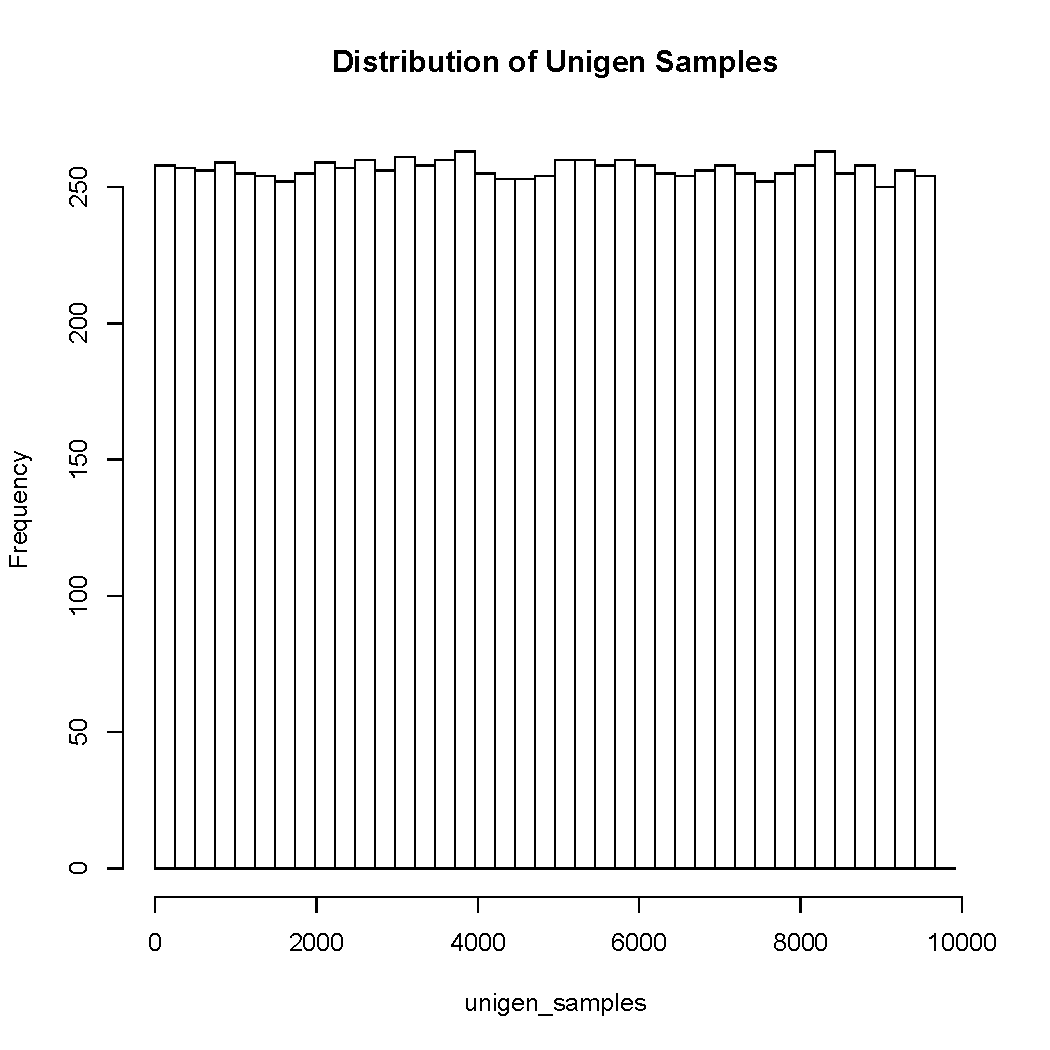
\includegraphics[origin=c,width=12cm]{../figures/unigen-samples.pdf}}
\caption{Distribution of Sequences Sampled by Unigen}
\label{fig:unigen_samples}
\end{figure}


\subsection{KUS}

% time python /home/drautb/GitHub/meelgroup/KUS/KUS.py --dDNNF d-DNNFs/stroop-3.dnnf --samples 10000 --outputfile d-DNNFs/stroop-3-kus-10000-samples.out
% ('Time taken to parse the nnf text:', 1.0481359958648682)
% ('Time taken for Model Counting:', 1.0421910285949707)
% ('Model Count:', 112409849997702614628L)
% ('Time taken by sampling:', 16.441092014312744)
% ('Samples saved to', 'd-DNNFs/stroop-3-kus-10000-samples.out')
% python /home/drautb/GitHub/meelgroup/KUS/KUS.py --dDNNF d-DNNFs/stroop-3.dnnf  25.76s user 0.59s system 102% cpu 25.828 total

KUS sampled 10,000 trials sequences, all of which were unique.

\begin{figure}[t]
\centering
\centerline{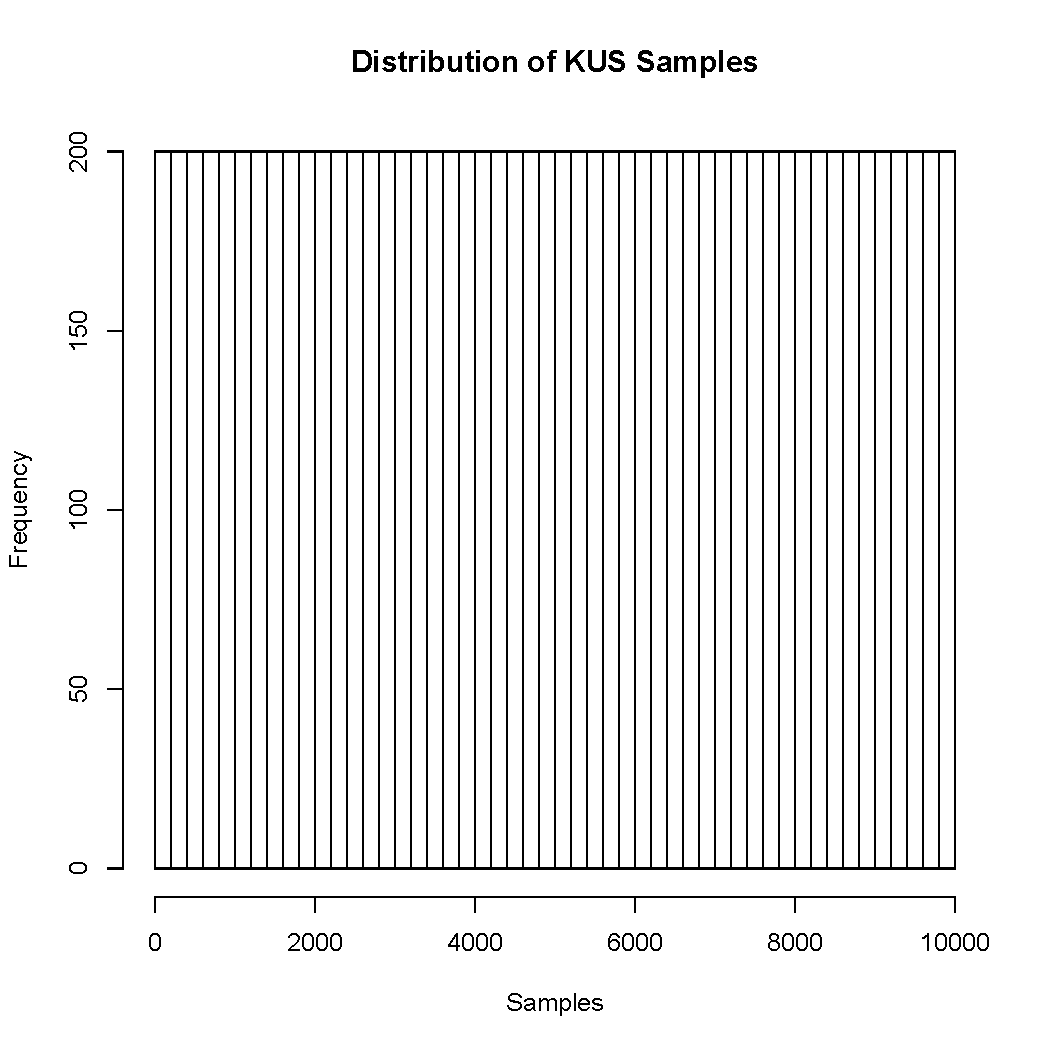
\includegraphics[origin=c,width=12cm]{../figures/kus-samples.pdf}}
\caption{Distribution of Sequences Sampled by KUS}
\label{fig:kus_samples}
\end{figure}


\subsection{Spur}

% time /home/drautb/GitHub/ZaydH/spur/build/Release/spur -q -s 10000 -cnf stroop-3.cnf -out stroop-3-spur-10000-samples.out
% /home/drautb/GitHub/ZaydH/spur/build/Release/spur -q -s 10000 -cnf  -out   30.97s user 0.23s system 99% cpu 31.250 total

Spur sampled 10,000 trial sequences, 9,664 of which were unique. 332 sequences were selected twice, and 2 were selected three times. No sequences were selected more than three times.

\begin{figure}[t]
\centering
\centerline{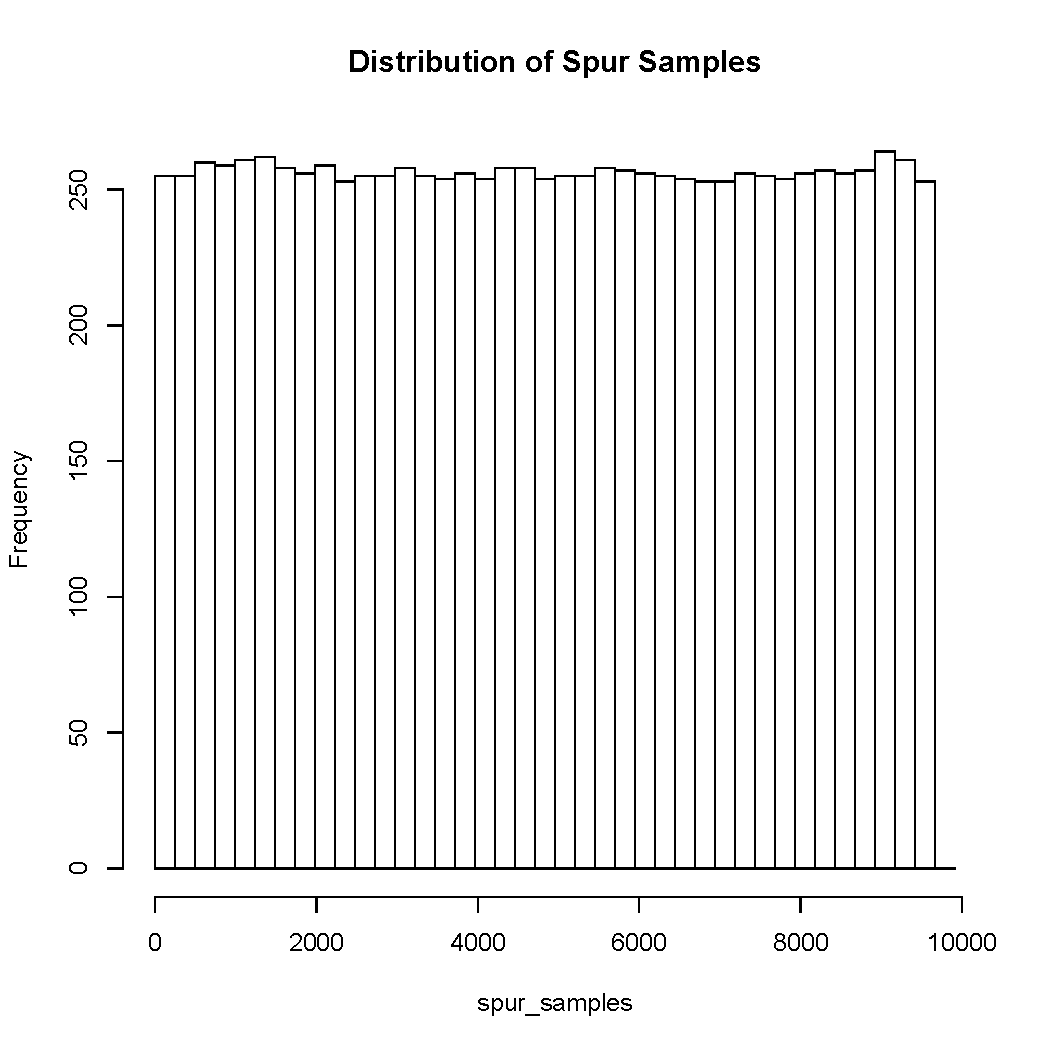
\includegraphics[origin=c,width=12cm]{../figures/spur-samples.pdf}}
\caption{Distribution of Sequences Sampled by Spur}
\label{fig:spur_samples}
\end{figure}


\subsection{CryptoMiniSat}

In contrast to the previous tests, when a SAT solver is used to generate individual samples incrementally by adding negated solutions to the prior formula, the same samples are generated each time. We used CryptoMiniSat to generate 10,000 samples as well, in groups of 100. Exactly the same set of 100 samples was generated each time.


\section{Summary}

We had hoped that Unigen would be able to sample from the space of solutions for experimental designs, in particular because the volume of variables and clauses in our generated CNF files fell within the range of example benchmarks provided by Unigen. However, the magnitude of the independent support set plays a critical role that was overlooked. Because the size of the independent support set for experimental designs grows quickly into the hundreds and thousands, a correspondingly large volume of \texttt{XOR} clauses is added to the CNF during sampling, which exceeds the capacities of the SAT solver (CryptoMiniSat). Furthermore, none of the additional tested tools for sampling SAT formulae are capable of handling the scale of practical experimental designs. Although the number of variables and clauses in the CNF for these experiments is reasonable, the factorial explosion in the number of solutions as well as the magnitude of the independent support set proved too large.
